\chapter{ACCS ADCOM 2019 Event Report}

\vskip -.5cm

\noindent\makebox[\textwidth]{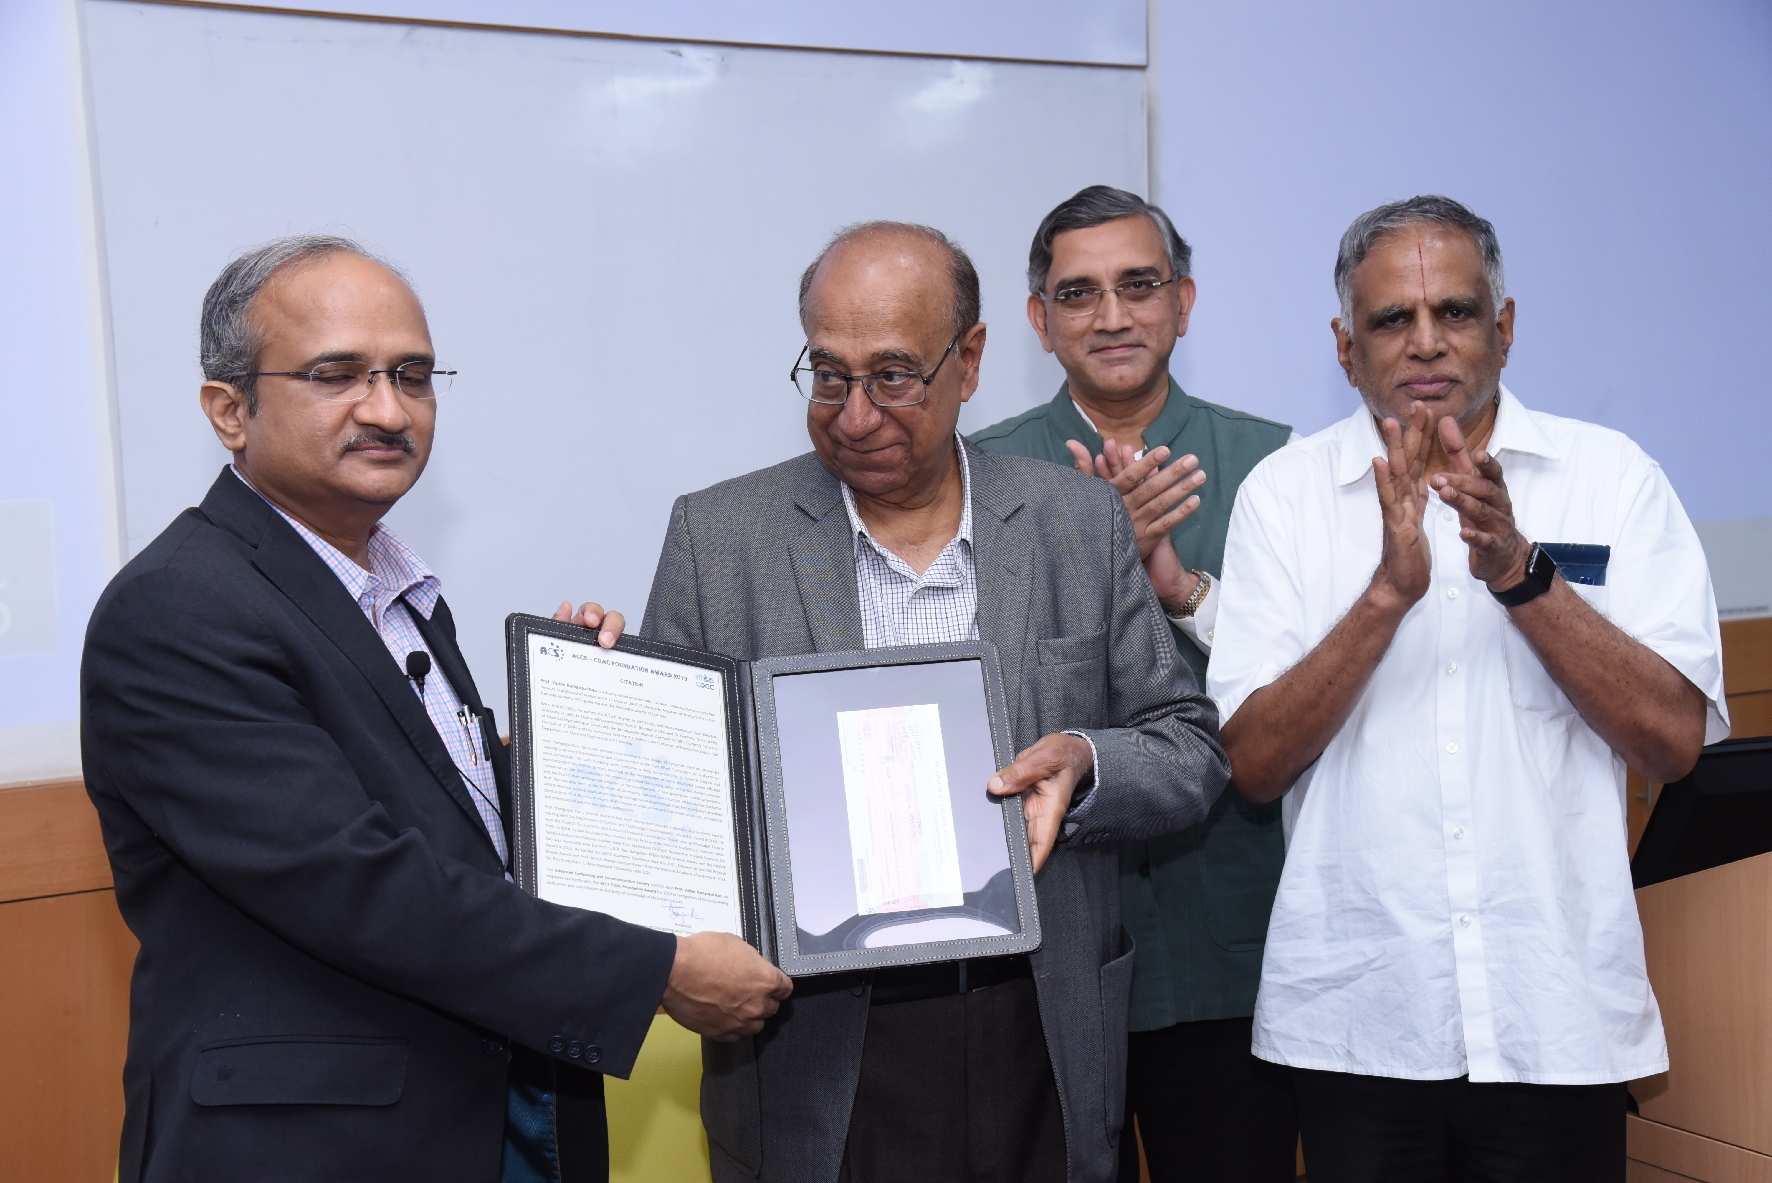
\includegraphics[width=\textwidth]{src/Figures/events/event-fig01.jpg}}

\vskip -.3cm

\begin{multicols}{2}
ACCS delivered its 25$^{\text{th}}$ edition of its flagship event - ADCOM 2019, earlier this month and there was higher anticipation of it being different from its previous editions. The event did not belie people’s expectations. Besides the high-profile keynote lectures, ACCS honored the doyens of Indian computing and communications science through the release of a Special Postal Cover by the Department of Posts, Government of India immortalizing the contributions of Late Dr. N. Seshagiri, Prof. V. Rajaraman, Dr. S. Ramani and Shri N. Vittal. Each one of them has strived in his own unique way to help build the Indian saga of computing and communications. For more on this, please see a special report on this event.

ADCOM 2019 explored the new generation of cellular and wireless communication, generally known as 5G (5$^{\text{th}}$ Generation). 5G promises to revolutionize wireless and mobile communication in innumerable ways giving rise to a new ecosystem and economy. A global roll out is underway in a phased manner yet many aspects of technical, infrastructural, policy matters are still evolving. It is in a way a giant leap for the communication industry which impacts every other segment of the society. The conference was held in Indian Institute of Information Technology-Bangalore (IIIT-B) from 5$^{\text{th}}$ September – 7$^{\text{th}}$ September, 2019. 

The highlight of ADCOM 2019 was of course the ACCS-CDAC Award 2019 conferred on Prof. V. Ramgopal Rao, Director of IIT-Delhi. Though this was on the second day, we will start this report from this key event.

\section*{The ACCS-CDAC 2019 Foundation Award Conferred}

Prof. V. Ramgopal Rao, joined 24 outstanding scientists and innovators in computing and communications to receive the prestigious ACCS-CDAC award for 2019. The award was established in 2004. Prof. Rao was chosen by the Selection Committee chaired by Prof. S. Sadagopan, Director of IIIT-B who said that the choice was unanimous. “Prof. Rao was recognized for this significant contribution in FinFETs making it possible to produce sub-10 nm microprocessors,” said Dr. Saragur Srinidhi, President of ACCS, reading the award citation. Prof. Rao is in the forefront of advanced investigations into making new inroads into nanoscale electronics. The award was conferred by the first recipient of the ACCS-CDAC Foundation Award, Dr. S Ramani, in the presence of Prof. S. Sadagopan and other eminent personalities from the field. 

\section*{Day 1: 5$^{\text{th}}$ September 2019}

\subsection*{Inaugural session}

\setcounter{figure}{0}
\begin{figure}[H]
\centering
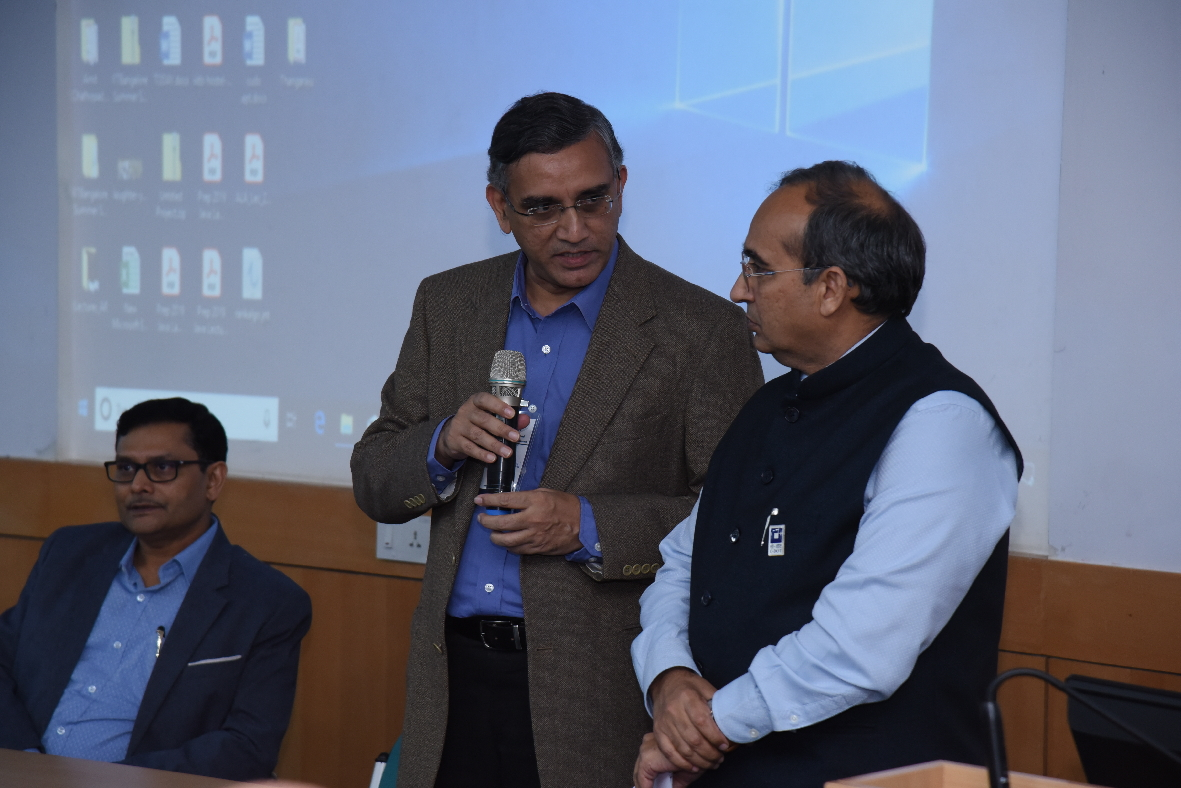
\includegraphics[scale=.88]{src/Figures/events/event-fig06.jpg}
\vspace{-2ex}
\end{figure}

The inaugural session of the ADCOM 2019 was chaired by Dr. Aloknath De, SVP \& CTO, Samsung Electronics and Dr.  Debabrata Das, HP Chair Professor - IIIT Bangalore. Dr. Saragur Srinidhi, President of ACCS, welcomed the gathering and introduced ACCS and ADCOM. This was followed by a video presentation from Professor Emeritus Arogyaswami Paulraj, Stanford University. Prof. Paulraj is a pioneer of MIMO wireless communications, a technology breakthrough that enables improved wireless performance. MIMO is now incorporated into all new wireless systems. In his video address, Prof. Paulraj likened the advent of 5G to the steam power in the 18$^{\text{th}}$ century, mass manufacturing in the 19$^{\text{th}}$ century and information technology in the 20$^{\text{th}}$ century. Prof. Paulraj who chaired the 5G Steering Committee setup by the Government of India gave insights into the report submitted by the committee that goes into the impact and touch points of 5G and infrastructural requirements. “5G will hugely transform India and for that we have make 5G affordable and pervasive,” he said. “It’s a lot of work and if we do it right, we will reap a One Trillion USD of economic value and this is a worthy cause to work for,” he added.

It was only apt that the entity which pioneered telematics innovation in India in the 80s, the Centre for Development of Telematics (C-DOT) present the 5G future in India. And Dr. Vipin Tyagi, CMD of CDOT gave the inaugural keynote. C-DOT is engaged in development of various projects at the frontier of Telecom technology in the areas of Optical communications, Next Generation Networks and Wireless technologies. 

\subsection*{Panel Discussion}

We had a lively panel discussion on, “Is leveraging 5G any different in developing nations than the developed ones?” moderated by Sanjiv Kovil, CTO Wipro with Dr. Aloknath De, CTO Samsung, Dr. Vipin Tyagi, ED C-DoT, Dr. Chandramouli Sargor, Head of Ericsson R\&D and Prof. Debabrata Das, IIITB in the panel. The panel went into the details of 5G roll out in the country, the standards or the lack of it, the infrastructural needs and finally the protocols and policies to enable the 5G ecosystem to thrive in India.

\vspace{-.3cm}

\noindent
\subsection*{Launch of Special Cover by Department of Posts}

\begin{figure}[H]
\centering
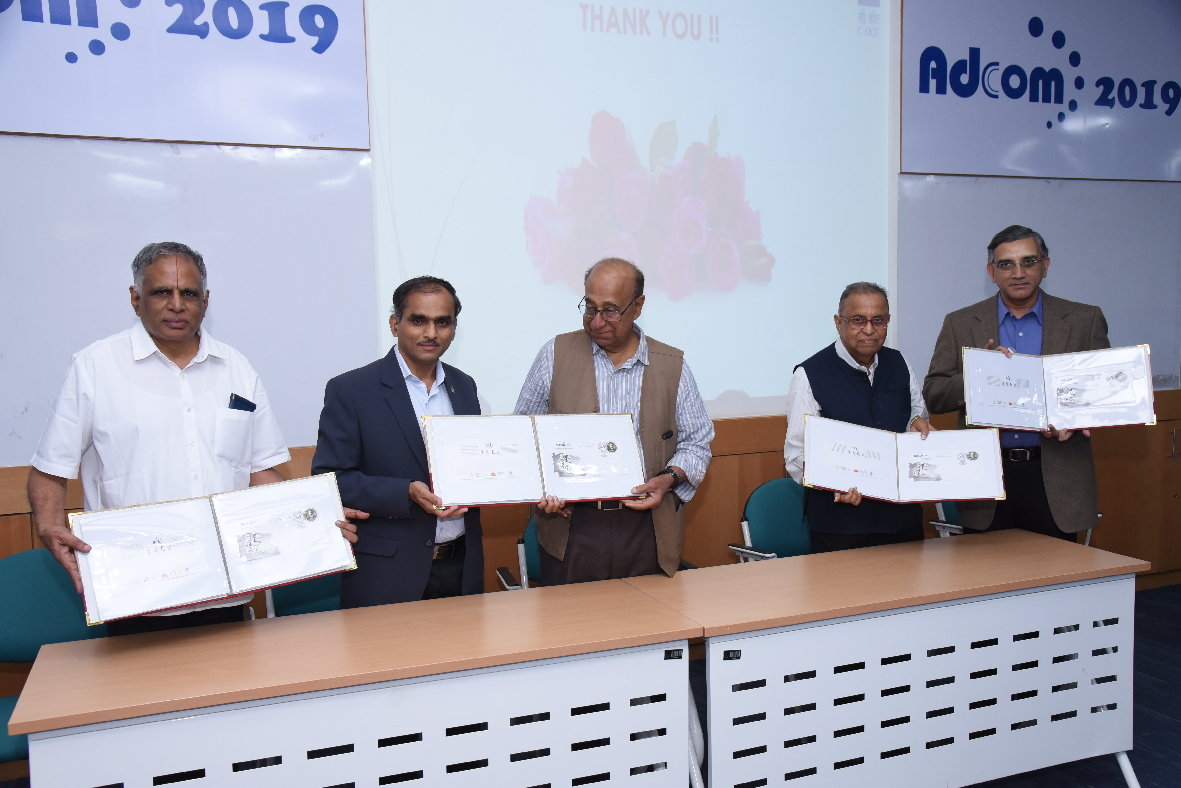
\includegraphics[scale=.88]{src/Figures/events/event-fig07.jpg}
\vspace{-2ex}
\end{figure}

The evening was marked by the release of a Special Postal Cover by Department of Posts, Government of India. Dr. Charles Lobo, Chief Postmaster General, Karnataka Postal Circle released the Special Postal Cover in the august presence of Prof. V. Rajaraman, Dr. S Ramani, Prof. S. Sadagopan, Dr. B.S. Sonde, Dr. S.K. Sinha and other eminent personalities. Dr. Ramani and Prof. Rajaraman were felicitated for their contributions to the field of computing and communications.

The morning of the first day saw enthusiastic students participating in a workshop on 5G Technology Development with Matlab, conducted by Ms. Vidya Viswanathan and Mr. Amod Jaiganesh from Mathworks. The students got a hands-on introduction on simulating various parameters and conditions using Matlab.

\section*{Day 2: 6$^{\text{th}}$ September 2019}

\begin{figure}[H]
\centering
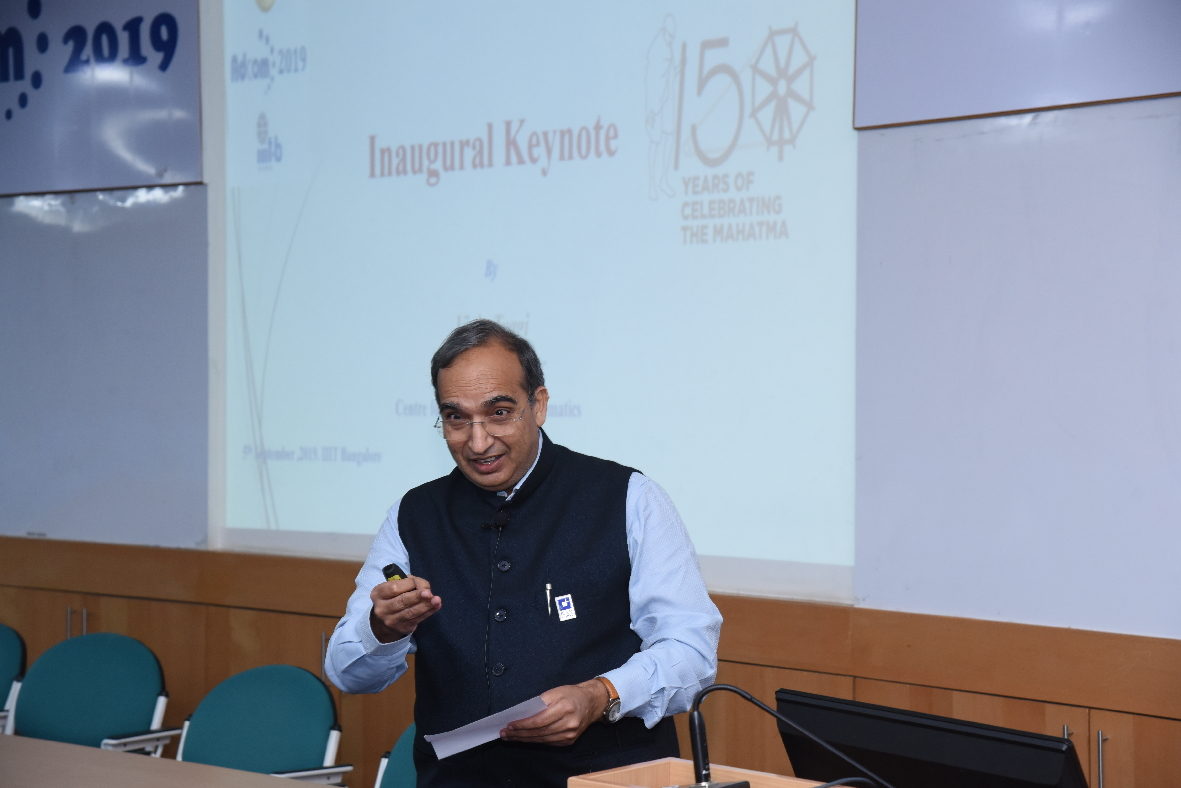
\includegraphics[scale=.88]{src/Figures/events/event-fig08.jpg}
\vspace{-2ex}
\end{figure}

The first keynote was by Mr. Satish Jamadagni of Reliance Industries who brings in over 20 years of industry experience in the telecom domain covering devices, networks, platforms and services. In his keynote on “5G Standards, where do we Stand?”, Mr. Jamadagni presented the immediate challenges facing the industry in terms of capacity and coverage, backhaul infrastructure, deployment flexibility, new service types and automation. The Industry is moving to adopt the 3GPP (3$^{\text{rd}}$ Generation Partnership Project) Release 17 Specification by the end of 2019. Mr. Jamadagni pointed out that the reign of LTE (Long Term Evolution), a 4G technology standard, will continue in the foreseeable future even as we hitch a ride on 5G.

Dr. Debarati Sen of the G.S. Sanyal School of Telecommunication, IIT-Kharagpur, delivered a keynote on, “Millimeter Wave (mmWave) Communication,” a field which was propounded by Indian scientist J.C. Bose, but coming into focus only now. Dr. Sen rightly started off her keynote with an \textit{ode} to the Bose, who had demonstrated millimeter wavelengths going upto 60 GHz to the Royal Society, London in 1919, 100 years ago. Dr. Sen touched upon the nature of MM wave communication, its application and how it dovetails with 5G ecosystem, channel models, beam forming methods and MM networks. Dr. Sen also laid out the future research in this field which includes Terahertz wavelength, Super Massive MIMO and AI techniques applied to MM communication.

Mr. Anshuman Nigam spoke on the readiness of 5G titled, “5G - It’s a Reality Now”. The immediacy of the message was not lost. Mr. Nigam is a Principal Architect, associated with Samsung R\&D Institute India, Bangalore (SRIB). Coming from a company which has aggressively pursued 5G technology, the keynote dwelt on some key developments, opportunities and roadmap. The road to 5G standardization is well on its way and by 2020 Tokyo Olympics, it is expected to reach application levels. Samsung itself is in test mode with its 5G enabled devices and will complete 5G Phase II roll out by December 2019. Mr. Nigam touched upon the migration path which leaps from the current 4G LTE standards to 5G NR (New Radio) and the impending launch roadmap. Most countries are 5G ready and operators have publicly announced roll out by end of 2019. He also dwelt upon the key features of 5G and how it promises just a quantum leap in almost every aspect of radio communication from bandwidth to privacy. 

Mr. Subhas Mondal's talk on, “Transformation of Industry with 5G” was spot-on. Mr. Mondal is driving the organization-wide 5G initiative as the chief architect at Wipro Ltd. Quoting Gartner that the 5G ecosystem will give rise to a \$1.3 Trillion economy by 2026, Mr. Mondal piqued the audience curiosity with the question, “Where is the Killer App.” There’s much promise around 5G from Gigabit in second to true AR/VR capability, machine to machine seamless communication to self-driving cars, which one will prove the golden goose for the advent of 5G? Mr. Mondal tried to separate the hype from the reality by bringing up several use cases that 5G enables and called for an Application Layer Standardization.

\vskip -.2cm

Dr. Dilip Krishnaswamy presentated on, “Distributed Processing In 5G Data Networks: A Convergence Of 5G, IoT, AI, and Blockchain,” which touched upon practicalities of distributed computing and processing in a networked world. Dr. Krishnaswamy talked at length on the trend towards disaggregation where monolithic systems will be broken down into Microservices and how Network Slicing will act as a key factor in dynamically disaggregating processing. He got into implementation details and painted a wonderful world that is about to be unleashed along with the advent of 5G networks. It is an interesting world emerging out there which takes the adage, “The Network is the Computer” to newer heights.  Dr. Krishnaswamy is currently serving as Vice President (New Technology Initiatives) at Reliance Jio Infocomm Ltd. His research interests include distributed information processing, distributed function virtualization, distributed resource management, block chain technology, edge services, NFV/SDN, NB-IoT, AI/ML, and 5G architecture \& systems. 

\subsection*{The Foundation Lecture}

The much anticipated ACCS Foundation Lecture was delivered by Prof. Ramgopal Rao, the recipient of this year’s ACCS - CDAC Foundation Award. While he went into the nuts and bolts of the world of sensors, Prof. Rao focused on how India is found to be best suited to play a major role in the oncoming an era of IoT devices powered by billions of sensors. He called on private industry, institutions and government agencies to work together to make India a \textit{sensor} innovation hub. Nanotechnology, Prof. Rao, said brings together the Physical science, Chemistry and Biological sciences together and India has an amazing talent pool which can dedicate itself on upcoming problem domains. India, he said, is in a unique position to give innovative sensor devices to the world.

\setcounter{figure}{0}
\begin{figure}[H]
\centering
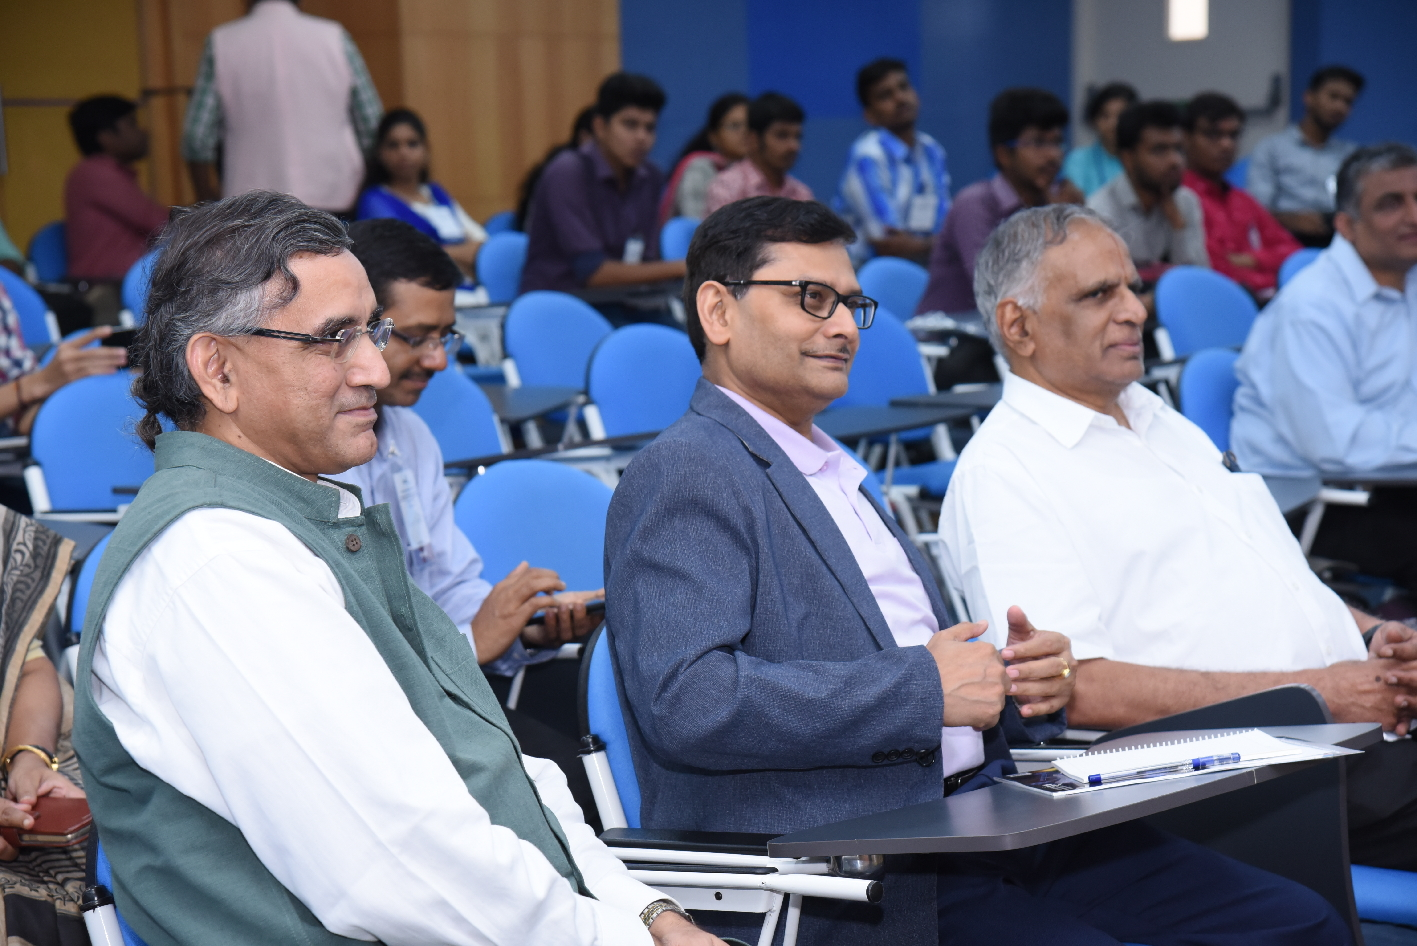
\includegraphics[scale=.75]{src/Figures/events/event-fig02.jpg}
\vspace{-4ex}
\end{figure}

In an interesting prelude to the Award ceremony, Mr. Jitendra Chaddah, Sr. Director, Operations and Strategy, Intel India, engaged Prof. Rao in a Fireside chat. The hour-long interaction ventured into Prof. Rao’s early career, his beginnings as a student, his interests and his amazing volume of work in which he has published over 400 papers and holds over 40 Patents in his name. Much of Prof. Rao’s work is in packing transistors on a chip more closely and yet avoiding the current leakage and other issues that come up when transistors are packed below 20 and 10 nm.

\begin{figure}[H]
\centering
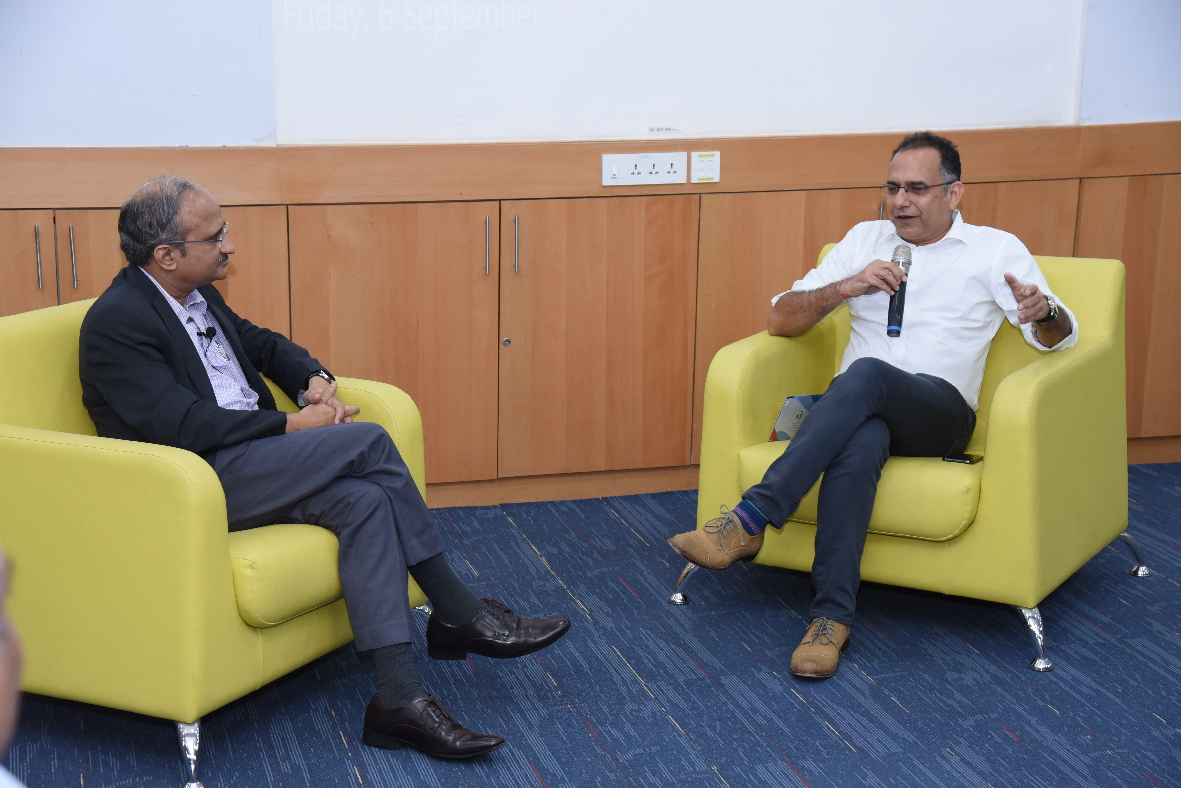
\includegraphics[scale=.9]{src/Figures/events/event-fig04.jpg}
\vspace{-2ex}
\end{figure}

\vspace{-.5cm}

\noindent
\subsection*{Student interaction}

Prof. Rao spent an hour interacting with Dr. Nanditha Rao and her students at IIITB discussing the state of research in India, how the youth can choose their path towards effective research work, what should Indian institutions to do to nurture an ecosystem for research and much more. 

\begin{figure}[H]
\centering
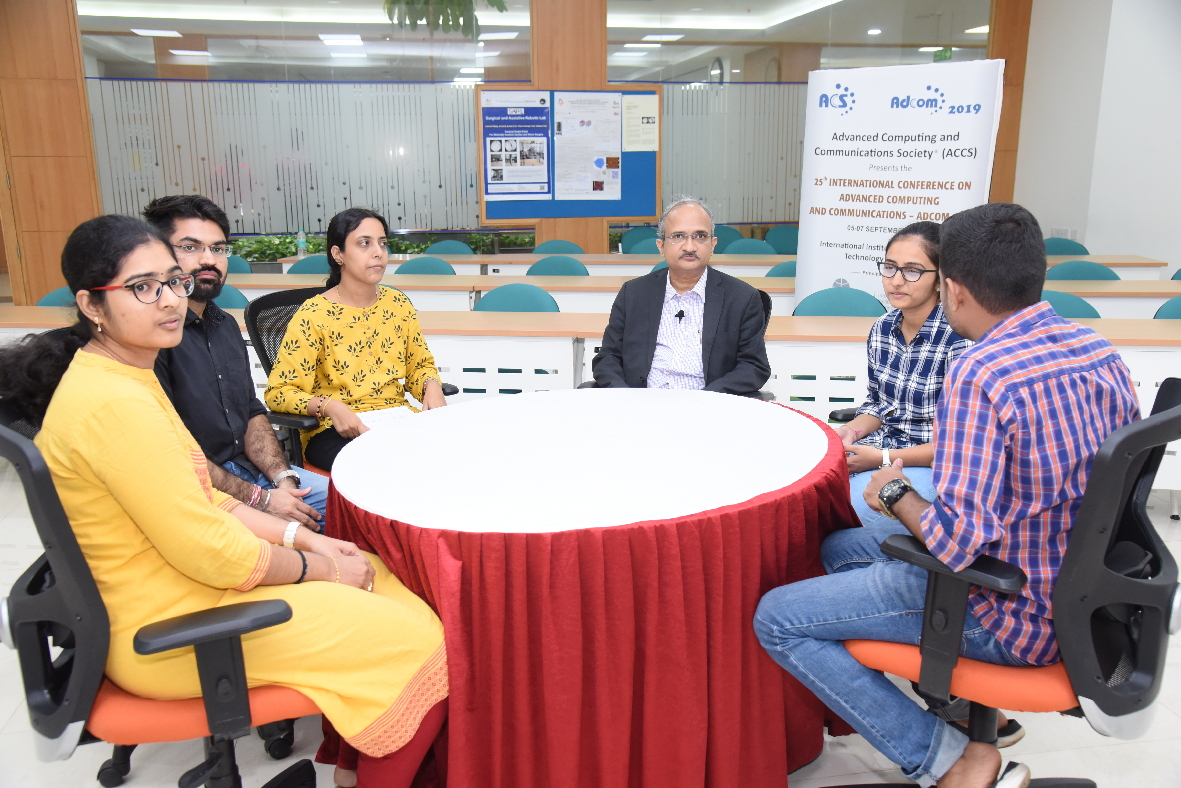
\includegraphics[scale=.9]{src/Figures/events/event-fig05.jpg}
\vspace{-2ex}
\end{figure}

\vspace{-.5cm}

\noindent
\subsection*{Ph.D. Forum and Technical Papers}

The PhD Forum@ADCOM is a short-paper session for PhD students to present and discuss their dissertation research with peers in the Computational and Communications Sciences. Some of the notable perr-reviewed papers were presented in the morning of Day 2 of the conference.


\section*{Day 3: 7$^{\text{th}}$ September 2019}

Second round of ACCS Design Challenge (ADC 2019), a collocated event, was held in which totally, 119 student-teams from 25 institutions participated. This was the 6$^{\text{th}}$ year for ADC. The presentations by the teams were reviewed by the Jury. Selected teams will enter the zonals.

The 25$^{\text{th}}$ edition of ADCOM was memorable in many ways. IIITB again was a wonderful host. Mr. Jailendra Kumar, Vice President of ACCS managed the sessions on both days. The students of IIITB had gracefully organized a Live Band on the evening of the second day which was followed by Conference Banquet. We had a host of student volunteers from the Global Academy of Technology who supported us on all days.

(ACCS Youtube Channel has videos of most of the sessions and keynotes, please visit \url{<link>})
\end{multicols}
